\documentclass{article}
\usepackage[utf8]{inputenc}
\usepackage[spanish]{babel}
\usepackage{graphicx}
\usepackage{anysize}
\usepackage{fancyhdr} 
\usepackage[export]{adjustbox}
\usepackage{titlesec}
\usepackage{enumitem}
\usepackage{amsmath}
\usepackage{amssymb}
\usepackage{listings}
\usepackage{xcolor}
% \usepackage{hyperref}
% \usepackage{float}
% \usepackage{tabu}

% Izquierda, derecha, arriba, abajo
\marginsize{1.5cm}{2cm}{1.2cm}{1cm} 
\renewcommand{\familydefault}{\sfdefault}
\decimalpoint%

\graphicspath{{assets/}{bdd_prac_06.assets/}}

\setlength{\parindent}{0in}
\titleformat*{\section}{\large\bfseries}

% Para insert código
\definecolor{codegreen}{rgb}{0,0.6,0}
\definecolor{codegray}{rgb}{0.5,0.5,0.5}
\definecolor{codepurple}{rgb}{0.58,0,0.82}
\definecolor{backcolour}{rgb}{1,1,1}

\usepackage{textcomp}
\lstset{upquote=true}
\lstdefinestyle{mystyle}{
    backgroundcolor=\color{backcolour},   
    commentstyle=\color{codegreen},
    keywordstyle=\color{magenta},
    numberstyle=\tiny\color{codegray},
    stringstyle=\color{codepurple},
    basicstyle=\ttfamily\footnotesize,
    breakatwhitespace=false,         
    breaklines=true,                 
    captionpos=b,                    
    keepspaces=true,                 
    % numbers=left,                    
    % numbersep=5pt,                  
    showspaces=false,                
    showstringspaces=false,
    showtabs=false,                  
    tabsize=2
}

\lstset{style=mystyle}

\newcommand{\materia}{BDD}
\newcommand{\clave}{2947}
\newcommand{\profesor}{Ing. Rodriguez Campos \textsc{Jorge Alberto}}
\newcommand{\grupo}{1}
\newcommand{\semestre}{2021-1}

\newcommand{\alumno}{
    Francisco Pablo \textsc{Rodrigo}  \\ 
    Flores Martinez \textsc{Emanuel}   
}

\newcommand{\actividad}{Práctica 06}
\newcommand{\titulo}{Transparencia de distribución - Mapeos locales}

\newcommand{\fechaEntrega}{6 diciembre de 2020}

\newcommand{\codedir}{bdd_prac_06-codigo}

%%%%%%%%%%%%%%%%%%%% ENCABEZADO %%%%%%%%%%%%%%%%%%%%%%%%%%%%
\pagestyle{fancy}
\fancyhf{}
\renewcommand{\headrulewidth}{0pt}
\fancyhead[R]{% Left header
    \begin{tabular}{l}
        \materia \\ 
        \actividad%
    \end{tabular}
    \,% Space
    \rule[-1.75\baselineskip]{0pt}{0pt}
    % Strut to ensure a 1/4 \baselineskip between image and header rule
    
\includegraphics[height=3\baselineskip,valign=c]{unam}
}
\setlength{\headsep}{0.3in}


\begin{document}
%%%%%%%%%%%%%%%%%%% DATOS PORTADA %%%%%%%%%%%%%%%%%%%%%%%%
\thispagestyle{empty}
\begin{minipage}[t][5cm][t]{0.2\linewidth}
    
\includegraphics[width=2.5cm]{unam.jpg}
    \vspace{10cm}

    
\includegraphics[width=2.5cm]{fiblack}
\end{minipage}
\begin{minipage}[t]{0.7\linewidth}
    \vspace{-2.5cm}
    \LARGE{\textbf{Universidad Nacional Autónoma de México}}\\
    \Large{\textbf{Facultad de Ingeniería}} \\

    \large{\semestre}\\[2cm]

    \large{\textbf{\materia (\clave)}}\\
    \large{\textbf{Gpo: 1}}\\[5mm]
    \large{\textbf{Profesor:} \profesor}\\ [1.5cm]
    \begin{center}
        \LARGE{\textbf{\actividad}}\\
        \LARGE{\textbf{\titulo}}\\
    \end{center}

    \vspace{3.3cm}

    % \large{\textbf{Alumno:} \alumno} \\[1.5cm]
    \large{
        \begin{itemize}[
            noitemsep,
            % topsep=0pt,
            % parsep=0pt,
            % partopsep=0pt,
            % labelwidth=5cm,
            align=left,
            % itemindent=2cm
        ]
            \item [\textbf{Alumno(s):}] 
            \begin{flushright}
                \alumno
            \end{flushright}
        \end{itemize}
    } \vspace{1.5cm}

    \begin{flushright}
        \fechaEntrega%
    \end{flushright}
\end{minipage}

\newpage
%%%%%%%%%%%%%%%%%%% CONTENIDO %%%%%%%%%%%%%%%%%%%%%%%%

\section*{Introducción}

En esta práctica se continuará con el caso de estudio que involucra 
suscriptores, revistas, articulos y pagos. Una vez que se tiene implementado
el esquema de fragmentación en cada PDB se debe empezar a implementar los
niveles de transparencia de distribución. A manera de recordatorio y en orden 
jerárquico se tiene: transparencia de fragmentación, transparencia de 
localización y transparencia de mapeos locales. \\

En esta práctica se implementarán mapeos locales dado que son los más básicos.
Para realizar dicha implementación se hará uso del concepto de ligas. Las
ligas son objetos que se guardan en la base de datos y que nos ayudan a 
realizar conexiones remotas sin la necesidad de utilizar la sentencia connect.
Es importante mencionar que para utilizar este nivel de transparencia es 
absolutamente necesario tener el listener en estado \textit{READY} ya que 
utilizaremos los servicios previamente configurados para formar la liga.

\section*{Objetivos}

Comprender la forma en la que se realiza la configuración de una base de datos 
Oracle para implementar el concepto de Transparencia de distribución en su 
primer nivel: Mapeos Locales. La implementación de este nivel se realizará a 
través del uso de PDBs y ligas (database links) para establecer una 
comunicación bidireccional.

\section*{C1. Diagrama Jerárquico }

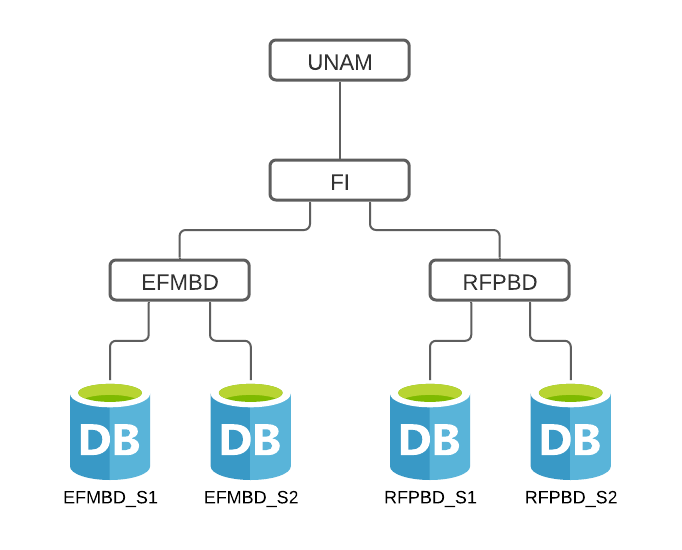
\includegraphics[width=\linewidth]{diagrama.png}

\section*{C2. Investigación modo dedicado/ modo compartido }

\subsection*{Configuración de una BD Oracle}

\subsubsection*{Modo dedicado}

\textbf{Descripción:} 
Se crea un proceso de servidor por cada usuario conectado a la base de datos. 
La información específica de cada proceso de servidor se guarda en la UGA 
(área dentro de la PGA) del usuario.\\

\textbf{Ventajas:}
\begin{itemize}
    \item Permite ejecutar operaciones que implican procesamiento de datos en batch.
    \item Permite emplear herramientas para realizar backups o recuperación 
      de la base de datos (RMAN).
    \item Útiles cuando las sesiones en las que la gran parte del tiempo están activas, 
    realizando múltiples operaciones dentro de la base de datos. \\
\end{itemize} 

\textbf{Desventajas:}
\begin{itemize}
    \item Usó de gran cantidad de recursos de la computadora.
\end{itemize}

\subsubsection*{Modo compartido}

\textbf{Descripción:} 
Un proceso de servidor compartido puede dar servicio a múltiples procesos de usuario. 
A cada petición se le asigna parte de la memoria compartida llama 
\textit{\textbf{virtual circuit}} empleado por el dispatcher para atender a cada petición
en la que se almacena información de las peticiones y respuestas del cliente. \\

\textbf{Ventajas:}
\begin{itemize}
    \item Cuenta con un \textit{dispatcher} que se encarga de administrar 
      los procesos de usuario.
    \item El número de procesos requeridos para administrar las peticiones es menor, 
      por lo que se consumen menos recursos.
    \item Cuando un proceso compartido está inactivo o no está siendo utilizado 
    por alguna sesión, este puede reutilizarse para atender otras peticiones. \\
\end{itemize} 

\textbf{Desventajas:}
\begin{itemize}
    \item Requiere que los clientes se conecten a la instancia a través de un 
      servicio de red (Net Service) sin importar que la petición sea local.
    \item El tiempo de ejecución de las sentencias puede ser mayor.
    \item La actividad del CPU puede aumentar por la actividad de las colas.
\end{itemize}

\section*{C3. Código únicamente para \texttt{suscriptor} y ejecución del 
  script \texttt{s-03-<SID>-consultas.sql}}

\lstinputlisting[language=SQL,firstline=33,lastline=45]
  {\codedir/s-03-efmbd_s1-consultas.sql}

%\textbf{Salida del script anterior}\\
  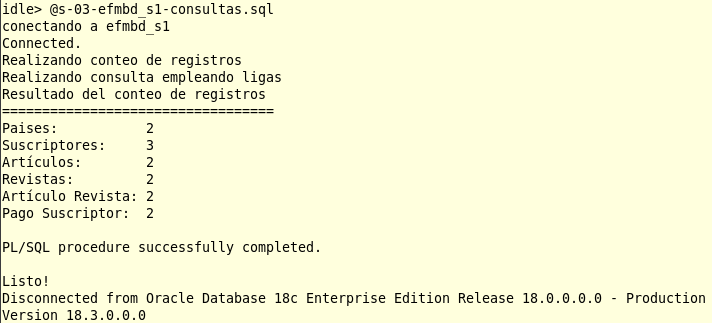
\includegraphics[width=0.8\linewidth]{efm_c3}

\lstinputlisting[language=SQL,firstline=35,lastline=49]
  {\codedir/s-03-rfpbd_s2-consultas.sql}

%\textbf{Salida del script anterior}\\
  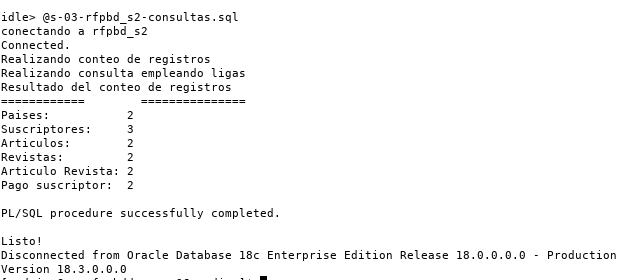
\includegraphics[width=0.8\linewidth]{rfp_c3}

\section*{C4. Actualización de fragmentos de código para el procedimiento 
  \texttt{guarda\_blob\_en\_archivo}}

  \lstinputlisting[language=SQL,firstline=66,lastline=91]
  {\codedir/s-00-guarda-blob-en-archivo.sql}

\section*{C5. Salida de ejecución del script de validación 
  \texttt{s-05-validacion-main.sql}}

  \subsection*{Salida de Francisco Pablo Rodrigo}

  \lstinputlisting[firstline=158]{bdd_prac_06-codigo/validador.txt}

  \subsection*{Salida de Flores Martínez Emanuel}

  \lstinputlisting[firstline=158]{bdd_prac_06-codigo/efm_validador.txt}

\section*{Comentarios y conclusiones}

En esta pŕactica aprendimos a trabajar con objetos binarios en nuestra base
de datos pero sobretodo dimos un gran repaso sobre las buenas prácticas
que debemos seguir a la hora de programar. De lo anterior podemos destacar la
importancia de comentar nuestro código, trabajar con sentencias preparadas
para evitar inyecciones SQL y por último, debemos sanitizar los parámetros
por medio de las funciones que normalmente ofrece cualquier lenguaje de
programación.\\

Por otra parte, con respecto de la materia, aprendimos como realizar el
nivel de transparencia de mapeos locales, el cual es el nivel más bajo de 
transparencia y tiene la desventaja de que el programador se encarga de todo:
realizar la reconstrucción de tablas en caso de que se pidan todos los 
datos de una determinada tabla, también es responsabilidad del programador 
cuidar la integridad al momento de realizar los inserts.\\

La práctica fue interesante, sin embargo, esperaba escribir el código de los
requerimientos planteados en los bullets, empero completar códgio nos ahorro
mucho tiempo.

\renewcommand\refname{Bibliografía}
\begin{thebibliography}{99}
    \bibitem{oracle} Oracle. \textit{Oracle Database Documentation} en 
        \texttt{https://docs.oracle.com/en/database/oracle/\\oracle-database/%
        index.html}
    \bibitem{oracledb} Oracle Database. \textit{Database PL/SQL Language 
        Reference} en 
        \texttt{https://docs.oracle.com/en/database/oracle/\\
        oracle-database/12.2/lnpls/database-pl-sql-language-reference.pdf}
\end{thebibliography}

\end{document}
